\documentclass[aspectratio=1610]{beamer}
\usepackage{tikz}
\PassOptionsToPackage{height=1.2cm}{beamerouterthemesidebar}

% Theme
\usetheme{LMS} % LMPS inspired


% packages 
\usecolortheme{default}
\usepackage{xcolor}
\usepackage{multicol}
\usepackage{multirow}
\newcommand\hmmax{0}
\newcommand\bmmax{0}
\usepackage{soul}

% My notations
\usepackage{MyNotations}





%%%%%%%%%%%%%%%%%%%%%% User commands %%%%%%%%%%%%%%%%%%%%%%
% To remove "Figure" from caption
\captionsetup{labelformat=empty,labelsep=none} 
\usefonttheme[onlymath]{serif}% Serif pour la police math

\usetikzlibrary{calc}
% https://tex.stackexchange.com/questions/601835/drawing-arrow-between-subfigures-in-scaleboxes

% To scale tikz figures from external files
\newcommand{\inputTikZ}[2]{%  
	\scalebox{#1}{\input{#2}}  
}

%% Data 
\title[] %optional
{\bfseries \textcolor{white}{Parametric implementation of Hierarchical Deep Learning Neural Network (HiDeNN)}
}
\subtitle{\itshape\textcolor{white}{ 1 parameter, 1D beam }}
%\author[A. Daby-S.] % (optional)
%{\textbf{\textcolor{BleuLMPS}{A.~Daby-Seesaram}} \\[47pt] \textcolor{BleuLMPS!80}{Supervised by D.~N\'eron, A.~Fau and P.-\'E.~Charbonnel} }



\date[VLC 2023] % (optional)
{\textcolor{white}{29$^{\text{th}}$ of February 2024}}


\begin{document}
	
	{
		%			\setbeamertemplate{background canvas}{bg=accentcolor}
		\setbeamertemplate{sidebar canvas left}{}
		\setbeamertemplate{sidebar left}{}
		\setbeamertemplate{background} 
		{	\hspace*{\sidebarwidth}
			\hspace{-1.9cm}
			
			%				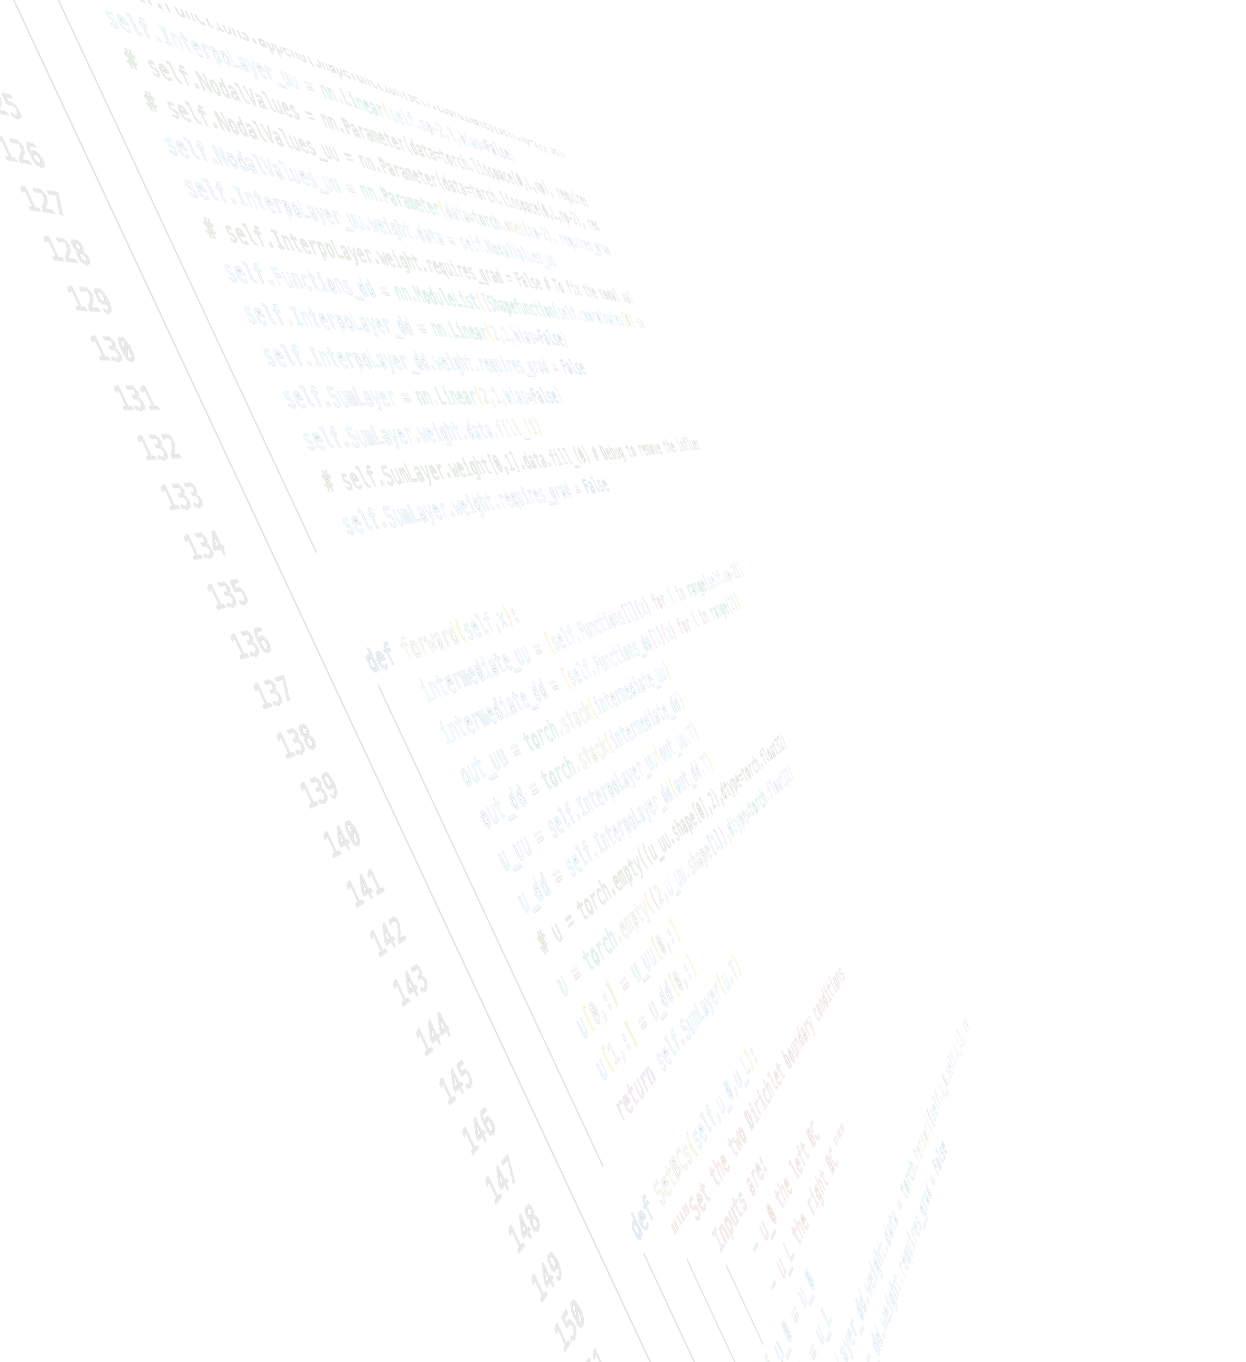
\includegraphics[width=\imagewidth]{Logos/LMS/Code_light.png}
			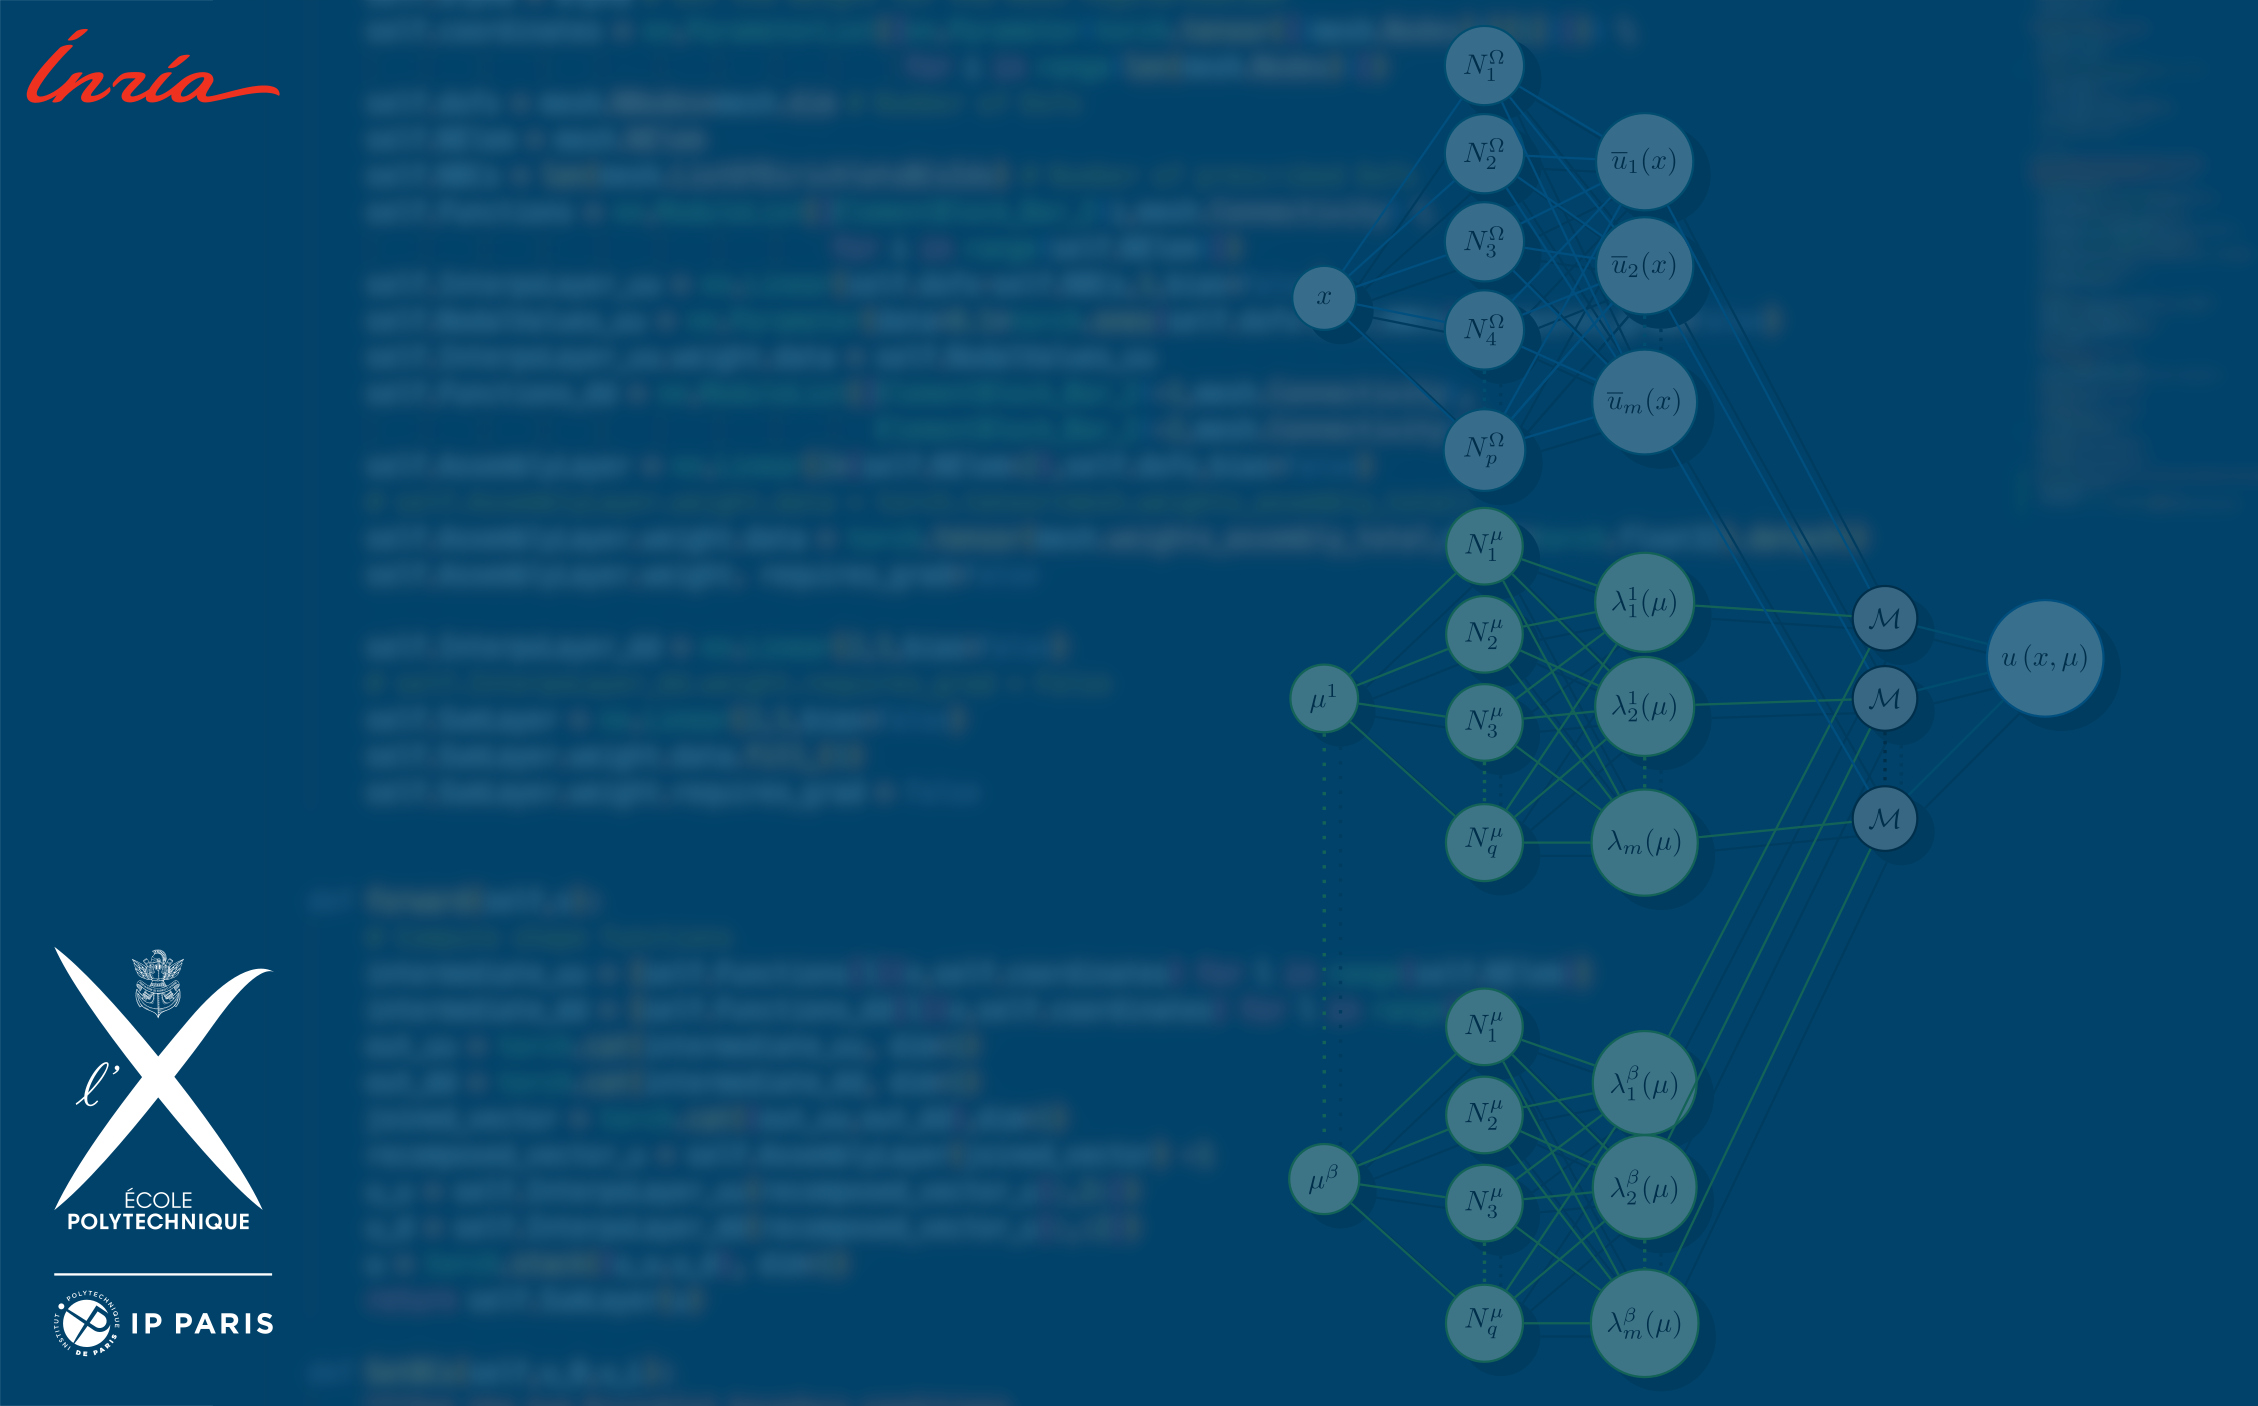
\includegraphics[width=1.121\imagewidth]{Logos/LMS/TitlePage.png}
		}
		
		\frame[plain]{\titlepage} 
	}
	
	
	
	%	
	
	%---------------------------------------------------------
	
	\section{Tensor decomposition}
	
	\begin{frame}
		\frametitle{\textsc{HiDeNN-PGD}}
		\framesubtitle{Uniform parameter}
		\begin{minipage}{0.48\linewidth}
			\begin{itemize}
				\item Tensor decomposition
				\begin{itemize}
					\item \small{$\displaystyle\vect{u}(\textcolor{BleuLMS!70}{\vect{x}},\textcolor{LGreenLMS}{\vect{\mu}}) = \sum\limits_{i=1}^m \textcolor{BleuLMS!70}{\overline{\vect{u}}_i(\vect{x})} ~\textcolor{LGreenLMS}{\lambda_i(\vect{\mu})}$} 
				\end{itemize}
				\item Illustration with $m=2$ 
				\item We already have the computation of $u_1(x)$
				\item $\left(p+q\right)\times m$ unknowns
				\item Achieve update by Freezing the $\left\{u_i\right\}_{i \in \llbracket 1,m \rrbracket}$
			\end{itemize}
		\end{minipage}
		\hfill 
		\begin{minipage}{0.48\linewidth}
			\centering
			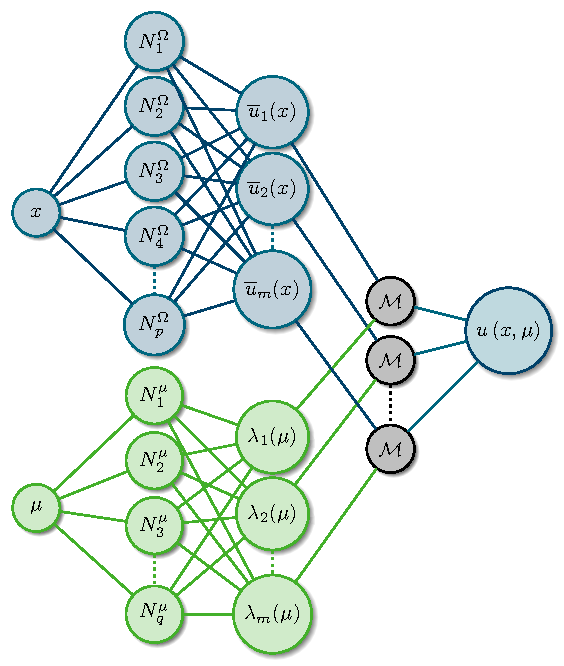
\includegraphics[width=\linewidth]{Schema/NN_TD_Scheme.pdf}
		\end{minipage}
	\end{frame}
	
	
	
	\begin{frame}
		\frametitle{\textsc{HiDeNN-PGD}}
		\framesubtitle{Spatial representation of the parameters}
		\begin{minipage}{0.58\linewidth}
			
			\begin{itemize}
				\item For a new patient, project $\mu\left(x\right)$ onto a basis $\left\{f^k\left(x\right)\right\}_{k \in \llbracket 1, \beta \rrbracket}$
				\begin{itemize}
					\item $\mu\left(x\right) = \sum\limits_{k=1}^{\beta}\mu^{k}f^k\left(x\right)$
					\item $\left\{u^k\right\}_{k \in \llbracket 1, \beta \rrbracket}$ input parameters for the NN
				\end{itemize}
				\item \small{$\displaystyle\vect{u}(\textcolor{BleuLMS!70}{\vect{x}},\textcolor{LGreenLMS}{\vect{\mu^1}, \cdots, \vect{\mu}^{\beta}}) = \sum\limits_{i=1}^m \textcolor{BleuLMS!70}{\overline{\vect{u}}_i(\vect{x})} ~\textcolor{LGreenLMS}{\prod_{j=1}^{\beta}\lambda_i^j(\vect{\mu^j})}$} 
				\item Retrieve $\mu\left(x\right)$ for computing the loss 
				\begin{itemize}
					\item $\mathcal{L} = g\left(\vect{u}\left((\textcolor{BleuLMS!70}{\vect{x}},\textcolor{LGreenLMS}{\left\{u^k\right\}}\right),\textcolor{BleuLMS!70}{\vect{x}},\mu\left(x\right)\right) $
				\end{itemize}
			\end{itemize}
			
		\end{minipage}
		\hfill 
		\begin{minipage}{0.38\linewidth}
			\centering
			
			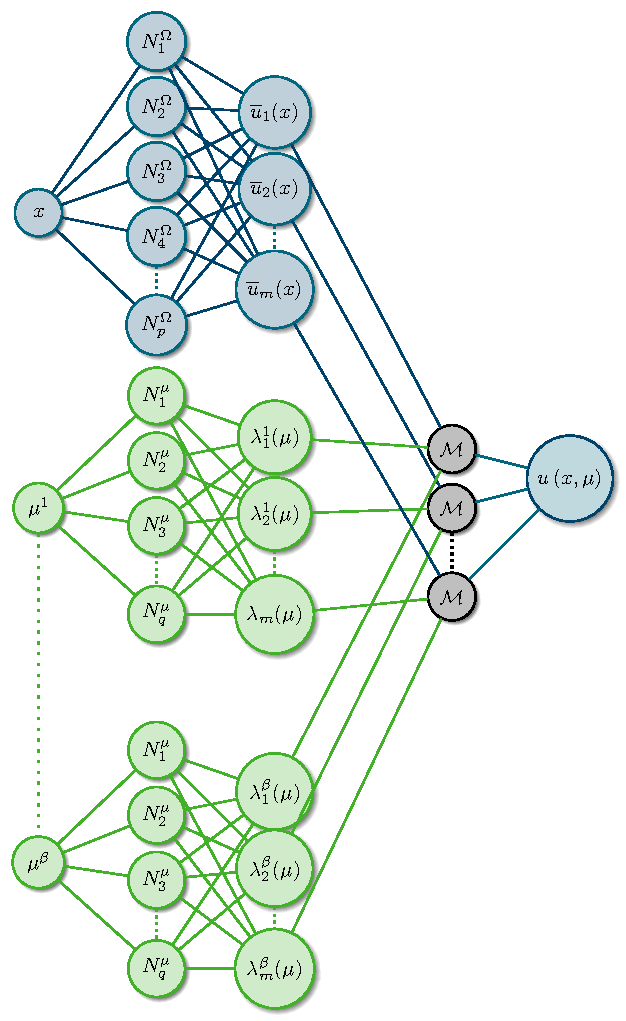
\includegraphics[width=\linewidth]{Schema/HiDeNN-TD-SpatialParam.pdf}
		\end{minipage}
	\end{frame}
	

	
\end{document}





